\documentclass[12pt]{article}
\usepackage[utf8]{inputenc}
\usepackage[spanish]{babel}
\usepackage[autostyle=false]{csquotes}
\MakeOuterQuote{"}
\usepackage{graphicx}
\usepackage{listings}
\usepackage[blocks]{authblk}
\newcommand{\email}[1]{\texttt{\small #1}}

\providecommand{\tightlist}{%
  \setlength{\itemsep}{0pt}\setlength{\parskip}{0pt}}


\title{Sistema Predictivo de Deserción Estudiantil}

\author{Juan Pablo Montesano\thanks{\email{jmontesano@antel.com.uy}}  
\quad Miguel Tasende\thanks{\email{mtasendebracco@antel.com.uy}} 
\quad Sebastián Laborde\thanks{\email{nlaborde@antel.com.uy}}}

\affil{Antel}

\begin{document}
\maketitle

\section{Introducción}
La deserción educativa es un gran problema en Uruguay, esta deserción del sistema educativo se instaló como un problema que atraviesa todas las clases sociales.\\
Entre las razones frecuentes de deserción encontramos dificultades en el aprendizaje, problemas de índole socio-económicos, ingreso temprano al mercado laboral, falta de interés del contenido pedagógico sumado a una preferencia por aprender cosas diferentes a las impartidas en los centros educativos, entre otras. Otra característica es que un alto porcentaje de quienes abandonaron el sistema educativo, había repetido al menos una vez algún curso, siendo los tres primeros años de escuela y primero de Ciclo Básico los años más frecuentes.\\
La motivación de esta propuesta, es la de dotar al sistema educativo de una herramienta que permita predecir el riesgo de deserción de los estudiantes del nivel básico y medio en el sistema educativo uruguayo. Mediante modelos predictivos es posible determinar patrones de comportamiento del alumno(a), analizando la historia académica del estudiante junto a los factores socio económicos y ambientales, que determinan su condición de potencial desertor, asociándolo un índice de deserción como probabilidad de abandono del sistema educativo.\\
A partir de este pronóstico, las autoridades gestoras del centro educativo y del sistema nacional podrían elaborar políticas de intervención efectivas y puntuales encaminadas a la retención de los alumnos y alumnas en el sistema educativo nacional (educación básica
y media) y al mejoramiento de los procesos de los centros educativos en pro de la disminución del índice de deserción escolar/liceal.\\
Nuestra idea es abordar el problema en un piloto que abarque un conglomerado de instituciones educativas primaria y media y que tengan similitudes socio-económicas, geográficas y ambientales, de forma que nuestro modelo predictivo se ajuste mejor a la realidad de los centros que estamos estudiando de lo que lo haría en un contexto más general con instituciones educativas que tuvieran realidades dispares. Es decir, cada conglomerado de un región escolar/liceal, debe ser considerada una población particular propensa de generar un modelo predictivo particular a partir de nuestro modelo macro.


\section{Diseño del sistema}
Existen varios enfoques diferentes para abordar los modelos predictivos de deserción, tentativamente proponemos utilizar el enfoque de reglas asociativas predictivas basado
en árboles de decisión y en reglas de dependencia que se definen a partir del contenido de información del modelo de datos de entrada y categorizan una serie de condiciones que se presentan de forma sucesiva. En esta técnica se identifican los árboles
de decisión binarios, random forest, gradient bossting, redes neuronales y otros.

Se propone utilizar un modelo estándar y una guía, estructurados en seis fases, algunas de estas fases son bidireccionales, lo que significa que algunas fases permitirán revisar
parcial o totalmente las fases anteriores.\\ Estas son:
\begin{itemize}
\item Entendimiento del problema
\item Comprensión de los datos
\item Preparación de los datos
\item Modelación
\item Evaluación del modelo
\item Despliegue o distribución del modelo.
\end{itemize}

Proponemos diseñar nuestro modelo para el ciclo de vida de un estudiante desde su inicio escolar hasta finalizar el liceo.

Para poder realizar un proceso de preparación de datos efectivo y de calidad partimos de un modelo de Deserción Escolar el cual lo representamos en el diagrama de estados (ver figura 1), cuyo objeto es establecer todos los posibles estados de un alumno(a) durante su tiempo de vida en el sistema educativo. Este modelo de estado nos provee los componentes
fundamentales para poder entender las condiciones iniciales, intermedias y finales del alumno inscrito en un centro educativo específico dentro del sistema educativo nacional. 

Nos va a servir para dos propósitos fundamentales: a) definir factores de medición o variables explicativas de la deserción escolar; b) establecer los procedimientos de preparación de los datos que van a servir de entrada al modelo predictivo de deserción escolar.


\begin{figure}[!h]
\centering
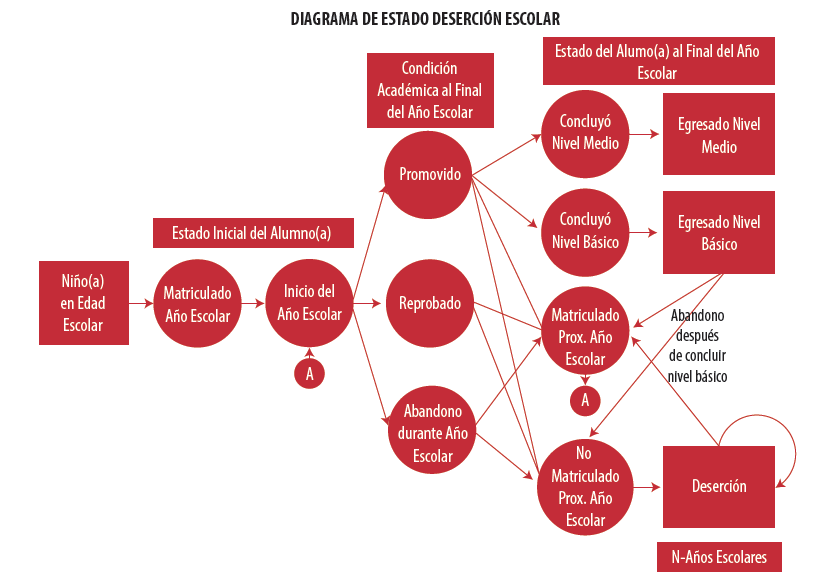
\includegraphics[width=4.0in]{diagrama_desercion.PNG}
\caption{Diagrama de estados de deserción escolar.}
\end{figure}

A partir de este modelo de estado del estudiante en el sistema educativo nacional podemos derivar un conjunto de mediciones que han de servir como parámetros
o factores explicativos de deserción escolar, en adición a los demás factores demográficos y socio económicos.

\section{Cómo funciona nuestro modelo predictivo}

El modelo predictivo cuenta de cuatro periodos en su ciclo de vida. Se selecciona un periodo de colección de datos o cohorte (historial de varios años académicos) que sirven de entrenamiento y prueba del modelo. Por ejemplo podemos usar 5 años 2013-2018 como periodo de cohorte, 70\% dataset de entrenamiento y 30\% dataset para prueba del modelo.

\begin{figure}[!h]
\centering
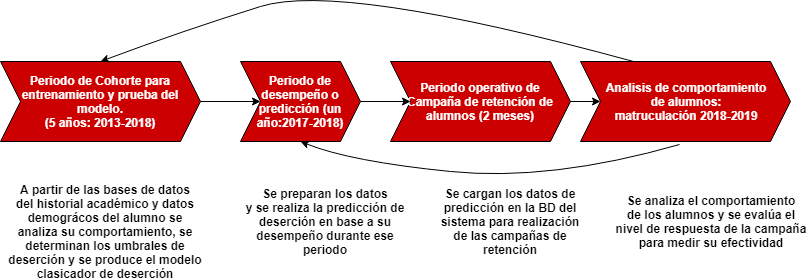
\includegraphics[width=6.0in]{model.png}
\caption{Ciclo de vida del Modelo.}
\end{figure}

Luego de la generación o entrenamiento del modelo basado en el algoritmo seleccionado se procede a observar su precisión y exactitud, tanto del set de entrenamiento como del de prueba, en una tabla de contingencia con pruebas estadísticas de significación (podemos utilizar F1 Score como medidas de precisión del modelo). Luego se procede a verificar el modelo simulando un periodo académico próximo, donde aplicaremos dichas prueba de igual manera. El próximo año académico se registra la matriculación del alumno y se contrasta con la predicción para ver el nivel de exactitud y precisión predictiva del modelo y como prueba de ajuste o desviación del modelo.\\

\begin{figure}[!h]
\centering
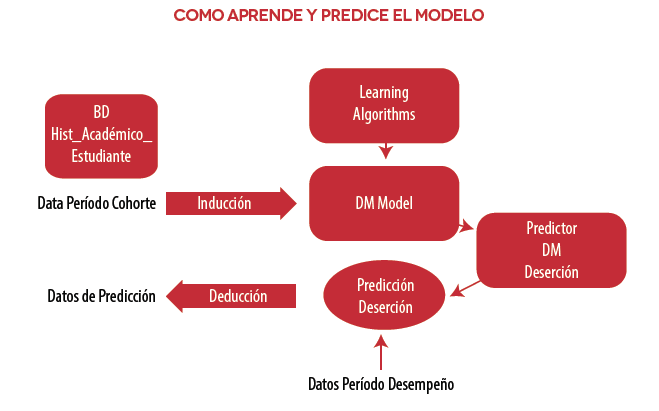
\includegraphics[width=6.0in]{learn.PNG}
\caption{Como aprende y predice el modelo.}
\end{figure}

Se usa el último año académico 2017-2018 como periodo de verificación del modelo simulando la predicción de este año basado en el entrenamiento de la cohorte seleccionada. Se proveen los datos de las variables explicativas con la condición de deserción en blanco, que es la variable a ser predicha.\\
El sistema proveerá un valor de cero o uno, según sea no o si la deserción esperada en la matriculación del siguiente año escolar 2018-2019. El valor del \% de confiabilidad será usado como valor en riesgo de la respuesta. Esta información deberá ser tenida en cuenta por los Centros Educativos con el objeto de servir a los planes de retención de alumnos con el mayor riesgo de deserción.

\end{document}